% AAAI-Style Two-Column Format (Custom Implementation)
% This uses standard packages to achieve AAAI-like formatting

\documentclass[letterpaper]{article}

% AAAI-like formatting
\usepackage[margin=1.75cm, top=2cm, bottom=2cm]{geometry}
\usepackage{times}
\usepackage{helvet}
\usepackage{courier}
\usepackage[hyphens]{url}
\usepackage{graphicx}
\urlstyle{rm}
\def\UrlFont{\rm}
\usepackage[numbers]{natbib}
\usepackage{caption}
\frenchspacing
\setlength{\pdfpagewidth}{8.5in}
\setlength{\pdfpageheight}{11in}

% Two-column layout
\usepackage{multicol}
\setlength{\columnsep}{0.5cm}

% Additional packages
\usepackage{amsmath,amssymb,amsfonts}
\usepackage{booktabs}
\usepackage{multirow}
\usepackage{tikz}
\usetikzlibrary{shapes,arrows.meta,positioning,fit,calc}
\usepackage{float}
\usepackage{hyperref}

% Title formatting (AAAI-like)
\makeatletter
\renewcommand{\maketitle}{%
  \begin{center}
    {\Large\bfseries \@title \par}
    \vspace{1em}
    {\normalsize \@author \par}
    \vspace{1.5em}
  \end{center}
}
\makeatother

% Section formatting
\usepackage{titlesec}
\titleformat{\section}{\normalfont\bfseries}{\thesection}{1em}{}
\titleformat{\subsection}{\normalfont\bfseries}{\thesubsection}{1em}{}
\titleformat{\subsubsection}{\normalfont\itshape}{\thesubsubsection}{1em}{}

\setcounter{secnumdepth}{2}

\title{Influencing the Divide: Political Polarization in Indian Influencer Discourse on X}

\author{
Ziv Barretto, Agriya Yadav, Kyra Chhetri, Anirban Sen\\
Ashoka University
}

\begin{document}

\maketitle

\begin{multicols}{2}

\begin{abstract}
This paper investigates partisan discourse on X (formerly Twitter), examining how political identities and affiliations shape online communication patterns. We analyze a large-scale dataset of tweets retweeted by Indian politicians from 2020-2023 to understand political polarization in social media. Our methodology combines influencer polarity scoring based on retweet behavior, automated keyword extraction using KeyBERT, and stance classification using a LoRA-adapted large language model. We identify politically polar keywords and classify tweet stances toward these topics to reveal patterns in how ruling and opposition parties engage with different political narratives.
\end{abstract}

\section{Introduction}

The rise of social media platforms has fundamentally transformed political communication and discourse. X (formerly known as Twitter) has emerged as a critical platform for political discussion, serving as a space where politicians, journalists, activists, and citizens engage in real-time conversations about political issues. However, this democratization of political discourse has coincided with growing concerns about political polarization and the formation of ideological echo chambers as pointed out by several recent research studies \cite{overgaard2024manifestation,pournaki2025influencers}.

This polarization has several detrimental effects on the information ecosystem, and the society at large. The lack of spread and cross-pollination of ideas across communities lead to unbalanced and incorrect judgment of social and political issues, thereby biasing electoral outcomes. The problem is further compounded by virality of mal-information and toxic content, resulting in an undesirable impact on democracy \cite{whatsappfake}.

More often than not, the boundaries of these echo chambers are fortified when the information is generated by a traditional influential figure (a prominent politician, business person, celebrity, etc.) with a significant network reach and follower count. 

Moreover, with the increasing accessibility of digital technologies, a second tier of micro-influencers (hereafter referred to as \textit{influencers}) has emerged as a significant contributor to polarization. Many of these individuals primarily derive their livelihoods from social media platforms and, in some cases, attain levels of popularity comparable to or exceeding those of traditional public figures. Content generated or disseminated by these influencers reaches a substantial audience, and consequently, ideological or opinion-based polarization among them further amplifies and compounds broader societal polarization. The political and social impact of these digital influencers can be estimated by the fact that influencer generated content accounted for around 36 \% of all user actions across major social platforms (Facebook, Instagram, X, TikTok) in April 2025, reflecting their mass global engagement \cite{socialsamosa2025influencerreport}. Political content alone drove over 30 \% of influencer interactions in India. Additionally, the influencer base seems to be ever-growing on social media, with India alone seeing a significant rise in number of influencers starting 2020 \cite{influencerrise}.

This paper investigates one of the axes of polarization among such influencers, namely the political axis. In other words, we study the partisan influencer discourse on X, examining if and how political leaning of influencers determine their online communication patterns on various social and political issues. The primary research question we intend to address in this work is: \textit{How does the political discourse of influencers on X vary on different social and political issues based on their political leaning?}

We currently focus on the Indian political context, although our methods are generalizable to any geography. We first develop a unique proxy for political leaning of influencers based on how politicians from the centrally ruling and opposition parties engage with their content. Next, we develop an \textit{Aspect based Stance Classifier} based on a small language model (\textit{Mistral-7B})\cite{jiang2023clip}, which analyzes the stance of the influencer tweets corresponding to the primary aspects/subjects contained in them. We also carry out our analysis separately for the tweets written in English and Hindi, to compare our findings across the linguistic spectrum.

Our findings empirically reveal that Indian influencers exhibit bipolar polarization with respect to a wide range of social and political issues, as identified by the aspects present in their tweets. Furthermore, an influencer’s political leaning is strongly correlated with the stance they adopt when tweeting on a given aspect. These observations raise several important questions and directions for future work, including how such polarization evolves over time, the mechanisms through which influencers shape and reinforce audience beliefs, and the extent to which polarized influencer discourse affects information diffusion and opinion formation among social media users. Future research could also investigate causal relationships between influencer stances and shifts in public opinion, as well as explore intervention strategies aimed at mitigating the amplification of polarization in social media ecosystems.

\section{Related Work}
Social media, lately, has become an indispensable source for news and information consumption \cite{pew_social_media_news_2025, toi_reuters_digital_news_india_2024} for the masses. A significant fraction of users stay updated with current affairs through social media, which leads to its impact on public opinion. Previous works report about this impact in various social and political fronts \cite{levy2021social,park2024exposure}, thereby conclusively proving that social media carries the power to reconfigure the very foundations of democracy. However, increasing polarization in social media has a detrimental impact on the society.  In this section, we discuss related work spanning the two primary components of our proposed framework -- analysis of social media polarization, and stance classification.

\subsection{Social Media Polarization}
While originally envisioned as a tool to broaden the horizons of knowledge and ideas, social media has contributed to an increasingly polarized and fragmented global society \cite{cicchini2022news,kofi_annan_social_media_polarization}. Polarization leads to imbalance in opinion formation, hindering individuals from obtaining a holistic view of salient issues. Numerous examples of the detrimental social impact causes by a polarized social media have been highlighted in prior studies [ref]. With the increasing penetration of digital technologies, policy-makers, think-tanks, and governments are increasingly planning necessary interventions to tackle the undesirable effect social media brings on the society \cite{oecd_facts_not_fakes_2024,carnegie_countering_disinformation_2024}. 

% One of the leading reasons behind social media polarization is the partisanship in the content posted by political entities. Previous studies have highlighted how social media was the key to achieving favorable electoral outcomes in the US presidential elections [ref]. Similar trends have been observed across the globe [ref], including the global south [ref] where increasing partisan content has led to significant polarization of the social media audience. The sources of such content are not just limited to political entities, but extend to traditionally influential figures like actors, athletes, and business-persons [ref]. 

Furthermore, the impact of polarization is often accentuated by \textit{micro-influencers} -- social media creators with dedicated following focused on a specific niche. These micro-influencers (or influencers) usually have a significantly high number of regular followers forming closely knit communities. Prior work has sufficiently exemplified cases where these influencers have promoted certain political agenda through highly partisan content posted through their social media accounts \cite{reinikainen2025convergence}. Owing to their network reach and impact, such content is consumed by their follower base, strengthening the pre-existing echo chambers. Similar trends have also been observed in India \cite{dash2022divided}, which forms the third highest user base for X, capturing around 36\% of all social media interactions globally across platforms \cite{socialsamosa2025influencerreport}.  

Social media polarization has been studied using both content \cite{falkenberg2022growing,nordbrandt2023affective,SUN2023113845} and network analysis methods \cite{esteve2022homophily,candellone2025negative,peralta2024multidimensional,singh2025multi,pournaki2025influencers,zhang2025polarization} in extant literature. %Falkenberg et al. \cite{falkenberg2022growing} study the discussion around the UN Conference of the Parties on Climate Change (COP) using Twitter data, and reveal a large increase in ideological polarization during COP26, contrary to the period between COP20 and COP25.  Overgaard et al. \cite{overgaard2024manifestation} measure affective polarization by looking at the expressed negativity towards certain actors through user comments. Maria Nordbrandt \cite{nordbrandt2023affective} uses Dutch panel data to show that the level of affective polarization affects subsequent use of social media. Sun et al. \cite{SUN2023113845} perform sentiment analysis of 3600 posts on Weibo, and find that content ideology and symbolic expressions are positively related to social media opinion polarization. Munoz et al. \cite{munoz2024quantifying} present a comparative analysis of polarization measurement methods on X during Spanish election cycles, and propose a novel algorithm for capturing polarization in political content.
The connection between partisanship in social media content and polarization has been well established in prior work. Demszky et al. \cite{demszky2019analyzing} use linguistic and semantic content analysis show that polarization is affected mainly by partisan differences in content framing. Flamino et al. \cite{flamino2023political} analyze tweets to examine how partisan news content circulated by media and influencer accounts increased ideological polarization between the 2016 and 2020 US elections. Dash et al. \cite{dash2022divided} quantify how influences engage with politically charged content in a partisan manner, showing that ideological polarization among influencers is linked to increased engagement and retweeting, thus amplifying partisan dynamics.

% Pournaki et al. \cite{pournaki2025influencers} measure political polarization by using topic modeling to identify issues and network analysis (Stochastic Block Models on retweet networks) to cluster users into global left-and right-leaning opinion camps. Zhang et al. \cite{zhang2025polarization} construct user opinion networks, and quantify polarization on social media through a random walk based approach.

Motivated by prior work in this area, we study the political discourse generated by Indian influencers to assess the level of partisanship in it. For this purpose, we first manually annotate a set of influencer generated tweets to create a dataset for aspect based stance classification. It is ensured that these tweets are politically endorsed, i.e., have been retweeted at least once by a political entity. Next, we use this dataset to fine-tune a small language model (Mistral-7B) to develop an aspect based stance classifier. While existing works have focused on various stance classification methods including XXX [ref], XXX [ref], and XXX [ref], we use an SLM based approach to ensure that our framework is generalizable to low resource settings. We also evaluate partisanism in influencer generated content in both English and Hindi, to establish robustness of our findings.
\subsection{Stance Classification}
Stance classification has long been recognized as a challenging NLP task involving the identification of a speaker’s holistic subjective disposition toward a topic or aspect. Prior work has shown that stance is not reducible to sentiment \cite{anand-etal-2011-cats}, and requires leveraging of significantly more nuanced linguistic features. Stance classification methods include both unsupervised \cite{gambini2022tweets2stance}, and supervised \cite{zarrella2016mitre,mohammad2017stance,xu2018cross,kuccuk2018stance} approaches. Prior work has shown that transformer-based approaches often substantially outperform classical approaches for stance detection on social media data \cite{glandt-etal-2021-stance,karande2021stance}. Recent work has additionally examined the use of LLMs for stance classification \cite{ding2024cross}, showing that LLM performance is highly sensitive to prompt design and that parameter-efficient fine-tuning such as LoRA does not consistently outperform zero-shot prompting \cite{cruickshank2023prompting,ma2024chain}. Prior work has also shown that effective stance classification requires rich representations and contextual modeling beyond surface lexical features \cite{hasan-ng-2013-stance}. Our work operationalizes these insights by extending this line of research to large-scale political influencer discourse, integrating LLM-based stance reasoning of multilingual tweet data. Specifically, we test the performance of both basic transformer and LLM based approaches (zero-shot, few-shot, and fine-tuned) in the task of stance classification, on influencer generated political tweets.

% TODO: Add literature review content

\section{Data Collection}

We utilize a dataset of tweets provided by Professor Joyojeet Pal, comprising retweets made by Indian politicians on X (Twitter) during the period 2020--2023. The dataset contains over 7.1 million retweet records, capturing the amplification behavior of politicians across the Indian political spectrum. Each record represents a retweet action containing the original tweet content, timestamp, retweeting politician's X handle, and the original author (influencer) whose content was retweeted.

To associate politicians with their party affiliations, we utilize an external mapping file containing X handles and corresponding party memberships. This mapping covers politicians from over 50 political parties, which we aggregate into two major blocs as shown in Table~\ref{tab:party_blocs}.

\vspace{0.5em}
\begin{center}
\footnotesize
\captionof{table}{Political Party Bloc Mapping}
\label{tab:party_blocs}
\begin{tabular}{p{3.2cm}p{3.2cm}}
\toprule
\textbf{Ruling Bloc} & \textbf{Opposition Bloc} \\
\midrule
BJP, JDU, LJP, HAM, JSP, NPP, AIADMK, AJSU, AGP, RPI, NPF, IPFT, NDPP, RSS, NDA, MNF, VHP, YSRCP, ABVP, BJD, BSCP & INC, AITC/TMC, DMK, SP, CPIM, RJD, AAP, JMM, IUML, CPI, NCP, TRS, Shiv Sena, TDP, JDS \\
\bottomrule
\end{tabular}
\end{center}
\vspace{0.5em}

The data processing pipeline consists of two stages. In the first stage (party labeling), we process the raw CSV in chunks of 100,000 rows and match each retweeting politician's handle to their party affiliation using lowercase normalization, producing a labeled dataset with the \texttt{retweet\_party} column. In the second stage (polarity calculation), we compute yearly polarity scores for each influencer based on who retweets their content, then average across years to obtain a stable polarity measure, identifying 960 unique influencers with calculable scores. Table~\ref{tab:dataset_stats} presents the key statistics of our dataset.

\vspace{0.5em}
\begin{center}
\small
\captionof{table}{Dataset Statistics}
\label{tab:dataset_stats}
\begin{tabular}{lr}
\toprule
\textbf{Metric} & \textbf{Value} \\
\midrule
Total retweets & 7,115,963 \\
English tweets & 2,939,716 (41.3\%) \\
Hindi/Regional tweets & 4,176,247 (58.7\%) \\
Unique influencers (with polarity) & 960 \\
Influencer-year observations & 3,712 \\
Temporal range & 2020--2023 \\
\bottomrule
\end{tabular}
\end{center}
\vspace{0.5em}

The temporal distribution (Table~\ref{tab:temporal_dist}) shows consistent activity across all four years, with relatively balanced influencer-year records ranging from 908 to 949 per year.

\vspace{0.5em}
\begin{center}
\small
\captionof{table}{Temporal Distribution of Tweets}
\label{tab:temporal_dist}
\begin{tabular}{lrr}
\toprule
\textbf{Year} & \textbf{Influencer-Year Records} \\
\midrule
2020 & 908 \\
2021 & 944 \\
2022 & 949 \\
2023 & 911 \\
\bottomrule
\end{tabular}
\end{center}
\vspace{0.5em}

Table~\ref{tab:columns} describes the key columns in our final processed dataset. The original dataset contains tweets in multiple languages, including Hindi and regional Indian languages. For the English analysis pipeline, we filter tweets using an ASCII-ratio heuristic: a tweet is classified as English if at least 85\% of its alphabetic characters are ASCII letters, providing computationally efficient language detection for large-scale processing.

\vspace{0.5em}
\begin{center}
\footnotesize
\captionof{table}{Dataset Column Descriptions}
\label{tab:columns}
\begin{tabular}{p{2.2cm}p{4.3cm}}
\toprule
\textbf{Column} & \textbf{Description} \\
\midrule
\texttt{timestamp} & Date and time of the retweet (UTC) \\
\texttt{tweet} & Full text content of original tweet \\
\texttt{retweet\_author} & X handle of retweeting politician \\
\texttt{original\_author} & X handle of influencer \\
\texttt{retweet\_party} & Political party of retweeter \\
\texttt{year} & Year extracted from timestamp \\
\texttt{side} & Political bloc (ruling/opposition/other) \\
\texttt{polarity\_avg} & Influencer's average polarity score \\
\texttt{tweet\_label} & Inferred political leaning of tweet \\
\bottomrule
\end{tabular}
\end{center}
\vspace{0.5em}

% \section{Methodology}

% \subsection{Influencer Polarity Calculation}

% A key insight of our approach is that politicians' retweet behavior reveals their political alignments. When a politician retweets content from an external account (influencer), it signals endorsement or amplification of that content. By aggregating retweet patterns across many politicians with known party affiliations, we can infer the political leaning of influencers.

% \subsubsection{Polarity Score Formulation}

% We first map all political parties to two major blocs: \textit{Ruling} (e.g., BJP, NDA coalition partners) and \textit{Opposition} (e.g., INC, TMC, AAP, and other INDIA bloc parties). For each influencer $i$ and year $y$, we calculate a yearly polarity score:

% \begin{equation}
% P_{i,y} = \frac{R_{i,y} - O_{i,y}}{R_{i,y} + O_{i,y}}
% \label{eq:polarity}
% \end{equation}

% \noindent where $R_{i,y}$ is the count of retweets the influencer received from Ruling bloc politicians in year $y$, and $O_{i,y}$ is the count from Opposition bloc politicians.

% The polarity score ranges from $-1$ (exclusively retweeted by Opposition) to $+1$ (exclusively retweeted by Ruling). We then compute an average polarity score across all available years for each influencer:

% \begin{equation}
% P_{avg,i} = \frac{1}{|Y_i|} \sum_{y \in Y_i} P_{i,y}
% \end{equation}

% \noindent where $Y_i$ is the set of years in which influencer $i$ was retweeted.

% \subsubsection{Classification Thresholds}

% Based on the average polarity score, influencers are classified into three categories:

% \begin{itemize}
%     \item \textbf{Pro-Ruling}: $P_{avg} \geq 0.5$
%     \item \textbf{Pro-Opposition}: $P_{avg} \leq -0.5$
%     \item \textbf{Neutral}: $-0.5 < P_{avg} < 0.5$
% \end{itemize}

% This classification is then propagated to all tweets authored by each influencer, labeling tweets based on the political leaning of their author.

% \subsubsection{Justification for This Approach}

% Alternative approaches to measuring political polarity include:
% \begin{itemize}
%     \item \textbf{Hashtag-based}: Inferring polarity from hashtag usage. However, hashtags can be appropriated, used sarcastically, or vary in political signal strength.
%     \item \textbf{Content-based}: Using sentiment analysis on tweet text. These methods struggle with context, sarcasm, and nuanced political language.
%     \item \textbf{Network-based}: Analyzing follower/following relationships. These are more stable but require extensive social graph data.
% \end{itemize}

% Our retweet-based approach leverages the revealed preferences of politicians---a retweet represents an explicit endorsement action, providing a more reliable signal than passive following or hashtag co-occurrence.

% \subsection{Keyword Extraction with KeyBERT}

% To identify the topics discussed in partisan discourse, we employ KeyBERT for automated keyword extraction from tweet text.

% \subsubsection{KeyBERT Methodology}

% KeyBERT uses sentence-level embeddings to identify keywords and phrases that are semantically similar to the document as a whole. The algorithm:

% \begin{enumerate}
%     \item Encodes the input document using a Sentence-BERT model
%     \item Generates candidate keywords/phrases
%     \item Encodes each candidate into the same embedding space
%     \item Ranks candidates by cosine similarity
%     \item Applies Maximal Marginal Relevance (MMR) for diversity
% \end{enumerate}

% \subsubsection{Configuration}

% We use the following configuration:

% \begin{itemize}
%     \item \textbf{Model}: \texttt{paraphrase-multilingual-MiniLM-L12-v2}
%     \item \textbf{N-gram range}: 1--2 (unigrams and bigrams)
%     \item \textbf{Top-N}: 3 keywords per tweet
%     \item \textbf{Diversity}: 0.7 (MMR parameter)
% \end{itemize}

% \subsubsection{Preprocessing}

% Before keyword extraction, tweets undergo preprocessing: URL removal, mention extraction (@ handles converted to tokens), hashtag segmentation (e.g., \texttt{\#AatmaNirbharBharat} $\rightarrow$ ``aatma nirbhar bharat''), and whitespace normalization.

% \subsubsection{Polar Keyword Selection}

% After extracting keywords from all tweets, we identify \textit{polar keywords}---topics that are disproportionately discussed by one political side. Keyword polarity is determined by analyzing the proportion of tweets from Pro-Ruling versus Pro-Opposition sources for each keyword.

% \paragraph{Initial Keyword Set (15 Keywords)}
% We first selected 15 keywords representing major political topics for manual annotation. These keywords were chosen based on their political significance and representation across both ruling and opposition discourse. Table~\ref{tab:polar_keywords} presents these keywords.

% \vspace{0.5em}
% \begin{center}
% \footnotesize
% \captionof{table}{Initial 15 Keywords for Manual Annotation}
% \label{tab:polar_keywords}
% \begin{tabular}{lp{2cm}}
% \toprule
% \textbf{Keyword} & \textbf{Dominant Side} \\
% \midrule
% caa & Pro-Opposition \\
% china & Mixed \\
% congress & Pro-Ruling \\
% farm\_laws & Pro-Opposition \\
% farmers\_protests & Pro-Opposition \\
% hindu & Pro-Ruling \\
% hindutva & Pro-Opposition \\
% kashmir & Mixed \\
% kashmiri\_pandits & Pro-Ruling \\
% modi & Pro-Ruling \\
% muslim & Pro-Opposition \\
% new\_parliament & Pro-Ruling \\
% rahulgandhi & Mixed \\
% ram\_mandir & Pro-Ruling \\
% shaheen\_bagh & Pro-Opposition \\
% \bottomrule
% \end{tabular}
% \end{center}
% \vspace{0.5em}

% \paragraph{Extended Keyword Set (23 Additional Keywords)}
% To expand coverage, we identified 23 additional polar keywords by analyzing tweet counts for each political bloc. Keywords were selected based on (1) clear partisan skew in usage patterns, and (2) relevance to significant political events or narratives. Table~\ref{tab:extended_keywords} presents a sample of these additional keywords with their extraction statistics.

% \vspace{0.5em}
% \begin{center}
% \footnotesize
% \captionof{table}{Sample Extended Polar Keywords with Extraction Stats}
% \label{tab:extended_keywords}
% \begin{tabular}{lrrr}
% \toprule
% \textbf{Keyword} & \textbf{Total} & \textbf{Pro-Ruling} & \textbf{Pro-Opp} \\
% \midrule
% ucc & 7,738 & 5,690 (74\%) & 2,048 \\
% democracy & 7,612 & 2,981 (39\%) & 4,631 \\
% mahotsav & 5,455 & 5,361 (98\%) & 94 \\
% aatmanirbhar & 5,386 & 5,289 (98\%) & 97 \\
% msp & 5,567 & 3,227 (58\%) & 2,340 \\
% sangh & 4,498 & 1,761 (39\%) & 2,737 \\
% ayodhya & 2,452 & 1,921 (78\%) & 531 \\
% unemployment & 1,649 & 284 (17\%) & 1,365 \\
% islamists & 1,488 & 1,470 (99\%) & 18 \\
% bhakts & 1,886 & 363 (19\%) & 1,523 \\
% \bottomrule
% \end{tabular}
% \end{center}
% \vspace{0.5em}

% The extended set includes keywords like \textit{aatmanirbhar} (self-reliance campaign), \textit{ucc} (Uniform Civil Code), \textit{ayodhya}, and \textit{mahotsav} which are predominantly used by Pro-Ruling sources (>74\%), while keywords like \textit{unemployment}, \textit{demonetisation}, \textit{bhakts}, and \textit{spyware} are predominantly discussed by Pro-Opposition sources (>80\%).

% \subsection{Stance Classification}

% To understand how different political factions discuss polar topics, we develop a stance classification system that determines whether a tweet expresses support, opposition, or neutrality toward a given keyword/entity.

% \subsubsection{Problem Formulation}

% Given a tweet $t$ and a target entity (keyword) $e$, the stance classification task predicts one of three labels:
% \begin{itemize}
%     \item \textbf{Favor}: Support for the entity
%     \item \textbf{Against}: Opposition to the entity
%     \item \textbf{Neutral}: No clear positive/negative stance
% \end{itemize}

% \subsubsection{Model Architecture}

% We employ a large language model (LLM) adapted for stance classification:

% \begin{itemize}
%     \item \textbf{Base Model}: Mistral-7B-Instruct, a 7-billion parameter instruction-tuned language model
%     \item \textbf{Adaptation}: Low-Rank Adaptation (LoRA), which freezes pre-trained weights and injects trainable rank decomposition matrices
% \end{itemize}

% LoRA enables parameter-efficient fine-tuning by decomposing weight updates into low-rank matrices:

% \begin{equation}
% W' = W + BA
% \end{equation}

% \noindent where $W$ is the frozen pre-trained weight matrix, and $B \in \mathbb{R}^{d \times r}$, $A \in \mathbb{R}^{r \times k}$ are trainable low-rank matrices with rank $r \ll \min(d, k)$.

% \subsubsection{Manual Annotation Process}

% For the initial 15 keywords, we manually annotated tweets to create training and evaluation data:


% \begin{enumerate}
%     \item \textbf{Sampling}: For each keyword, we sampled 100--150 tweets, balancing Pro-Ruling and Pro-Opposition sources
%     \item \textbf{Deduplication}: Removed duplicate tweets and near-duplicates to ensure annotation quality
%     \item \textbf{Labeling}: Each tweet was labeled with stance (favor/against/neutral) and a brief reasoning
%     \item \textbf{Consolidation}: Annotations were organized into per-keyword files
% \end{enumerate}

% The final annotated dataset comprises 1,866 labeled tweet-keyword pairs across 15 keywords.

% \subsubsection{Training and Evaluation Split}

% The annotated data was split 85:15 for training few-shot examples and held-out evaluation, using stratified sampling to maintain class balance across keywords.

% \begin{itemize}
%     \item \textbf{Training set}: 10 examples per keyword (3 favor, 3 against, 3 neutral, 1 filler) used as few-shot prompts
%     \item \textbf{Test set}: 264 samples for evaluation
% \end{itemize}

% \subsubsection{Few-Shot Inference}

% During inference, the system dynamically retrieves keyword-specific few-shot examples to construct the prompt. If keyword-specific examples are unavailable (for the extended 23 keywords), the system falls back to a global set of examples, enabling stance classification across all 38 keywords.

% \subsubsection{Output Format}

% The model generates structured JSON output:

% \begin{verbatim}
% {
%   "stance": "favor|against|neutral",
%   "reason": "<brief explanation>"
% }
% \end{verbatim}

% \subsubsection{Model Evaluation}

% We evaluated the LoRA-adapted model on the held-out test set of 264 samples. Table~\ref{tab:eval_overall} presents the overall classification performance.

% \vspace{0.5em}
% \begin{center}
% \footnotesize
% \captionof{table}{Stance Classification Evaluation Results}
% \label{tab:eval_overall}
% \begin{tabular}{lr}
% \toprule
% \textbf{Metric} & \textbf{Value} \\
% \midrule
% Total test samples & 264 \\
% Accuracy & 78.0\% \\
% Precision (macro) & 78.0\% \\
% Recall (macro) & 75.3\% \\
% F1-Score (macro) & 76.2\% \\
% F1-Score (weighted) & 77.7\% \\
% \bottomrule
% \end{tabular}
% \end{center}
% \vspace{0.5em}

% Table~\ref{tab:eval_perclass} shows the per-class performance breakdown.

% \vspace{0.5em}
% \begin{center}
% \footnotesize
% \captionof{table}{Per-Class Classification Performance}
% \label{tab:eval_perclass}
% \begin{tabular}{lrrrr}
% \toprule
% \textbf{Class} & \textbf{Precision} & \textbf{Recall} & \textbf{F1} & \textbf{Support} \\
% \midrule
% Against & 0.78 & 0.80 & 0.79 & 95 \\
% Favor & 0.78 & 0.86 & 0.82 & 111 \\
% Neutral & 0.78 & 0.60 & 0.68 & 58 \\
% \bottomrule
% \end{tabular}
% \end{center}
% \vspace{0.5em}

% The model achieves strongest performance on the ``favor'' class (F1=0.82), followed by ``against'' (F1=0.79). The ``neutral'' class shows lower recall (0.60), reflecting the inherent difficulty in distinguishing neutral stances from weakly expressed opinions.

% Table~\ref{tab:eval_keyword} presents per-keyword accuracy, showing variation across different political topics.

% \vspace{0.5em}
% \begin{center}
% \footnotesize
% \captionof{table}{Per-Keyword Classification Accuracy (Top 10)}
% \label{tab:eval_keyword}
% \begin{tabular}{lrr}
% \toprule
% \textbf{Keyword} & \textbf{Accuracy} & \textbf{F1 (macro)} \\
% \midrule
% modi & 94.4\% & 0.91 \\
% caa & 89.5\% & 0.90 \\
% congress & 88.9\% & 0.84 \\
% hindutva & 85.7\% & 0.56 \\
% new\_parliament & 85.7\% & 0.82 \\
% rahulgandhi & 81.3\% & 0.81 \\
% farmers\_protests & 80.0\% & 0.82 \\
% shaheen\_bagh & 78.9\% & 0.71 \\
% muslim & 78.9\% & 0.79 \\
% china & 73.7\% & 0.64 \\
% \bottomrule
% \end{tabular}
% \end{center}
% \vspace{0.5em}

\section{Methodology}

\subsection{Influencer Polarity}
We calculate an influencer's political leaning (also termed as \textit{polarity}) using the amount of endorsement their tweets receive from Indian politicians. Generally, the retweet behavior of politicians reveals their endorsement towards a tweet [ref]. Thus, by aggregating retweet patterns across politicians with known party affiliations, we can infer the political leaning of influencers. This methodology provides a more reliable signal of endorsement than passive following or hashtag co-occurrence, since hashtags can be appropriated or used sarcastically, while generic sentiment analysis methods struggle with political nuance and sarcasm.

For each influencer $i$ and year $y$, we calculate a yearly political polarity score using the formula in Equation~\ref{eq:polarity} where $R_{i,y}$ represents the count of retweets the influencer received from ruling politicians in year $y$, and $O_{i,y}$ represents the count from opposition politicians.

\begin{equation}
P_{i,y} = \frac{R_{i,y} - O_{i,y}}{R_{i,y} + O_{i,y}}
\label{eq:polarity}
\end{equation}

The polarity score ranges from $-1$ (exclusively retweeted by opposition) to $+1$ (exclusively retweeted by ruling). %The computation involves grouping data by influencer, year, and political side, then pivoting to create ruling and opposition columns with missing values filled as zero.
We next compute an average polarity score across all available years using Equation~\ref{eq:polarity_avg}, where $Y_i$ is the set of years in which influencer $i$ was retweeted by at least one politician.

\begin{equation}
P_{avg}^i = E_y[P_{i,y}] = \frac{1}{|Y_i|} \sum_{y \in Y_i} P_{i,y}
\label{eq:polarity_avg}
\end{equation}

Based on the average polarity score, influencers are classified into three categories using a threshold of 0.5 (experimentally determined). Influencers with $P_{avg}^i \geq 0.5$ are classified as Pro-Ruling, those with $P_{avg}^i \leq -0.5$ as Pro-Opposition, and those within $-0.5 < P_{avg}^i < 0.5$ as Neutral. This classification is propagated to all tweets authored by each influencer, effectively labeling tweets based on their author's political leaning.

Three independent annotators also manually analyzed the influencer polarities to validate the results. This exercise reached a high inter-annotator agreement (95\% unanimous agreement), revealing the above-par performance of the procedrure.

\subsection{Aspect Identification}
To identify the topics or aspects discussed in influencer tweets, we employ KeyBERT\cite{grootendorst2020keybert} for automated keyword extraction from tweet text. KeyBERT leverages BERT embeddings to identify keywords and phrases that are semantically similar to the document as a whole, making it suitable for capturing the topical essence of short-form social media content.

Before aspect extraction, we preprocess the tweets to remove URLs, strip the "@" character while retaining usernames, perform hashtag segmentation using the \texttt{wordsegment} library (e.g., \texttt{\#AatmaNirbharBharat} becomes \textit{aatma nirbhar bharat}), and normalize whitespaces.

The extraction process uses the \texttt{paraphrase-} \texttt{multilingual-MiniLM-L12-v2} sentence transformer model as the KeyBERT backend. We configure n-gram range of 1--2, extract top three aspects per tweet, and apply Maximal Marginal Relevance (MMR) with diversity 0.7 to balance semantic similarity with keyword diversity.

\textbf{Polar Aspect Identification:} To understand if influencers with a certain political polarity preferentially tweet around certain political aspects, we analyze the aspects to identify \textit{polar aspects} -- topics disproportionately discussed by one political side. We first manually selected 15 aspects representing major political topics for annotation, chosen based on their political significance and representation across both ruling and opposition discourse. We examined the proportion of tweets from pro-ruling and Pro-Opposition sources for each selected aspect, and categorize the aspect as pro-ruling/opposition based on which side tweets more about it. This forms the seed set of polar aspects. Next, to expand coverage, we systematically analyzed aspect frequencies and identified 23 additional polar aspects exhibiting clear partisan skew. Table~\ref{tab:all_keywords} presents the complete set of 38 keywords used for stance analysis.
\begin{center}
\footnotesize
\captionof{table}{Complete Keyword Set for Stance Analysis}
\label{tab:all_keywords}
\begin{tabular}{llll}
\toprule
\multicolumn{4}{c}{\textbf{15 seed aspects identified manually}} \\
\midrule
caa & congress & farm\_laws & farmers\_protests \\
hindu & hindutva & kashmir & kashmiri\_pandits \\
modi & muslim & new\_parliament & rahulgandhi \\
ram\_mandir & shaheen\_bagh & china & \\
\midrule
\multicolumn{4}{c}{\textbf{23 extended aspects identified using frequency analysis}} \\
\midrule
aatmanirbhar & ayodhya & balochistan & bhakts \\
democracy & demonetisation & dictatorship & gdp \\
hathras & inflation & islamists & lynching \\
mahotsav & minorities & msp & ratetvdebate \\
sangh & sharia & spyware & suicides \\
ucc & unemployment & & \\
\bottomrule
\end{tabular}
\end{center}
Aspects like \textit{aatmanirbhar} (self-reliance campaign), \textit{ucc} (Uniform Civil Code), \textit{ayodhya}, and \textit{mahotsav} are predominantly used by Pro-Ruling sources ($>74\%$), while \textit{unemployment}, \textit{demonetisation}, \textit{bhakts}, and \textit{spyware} are predominantly discussed by Pro-Opposition sources ($>80\%$).
\subsection{Stance Classification}
The goal of our stance classification system is to determine how influencers position themselves toward specific political topics. Given a tweet $t$ and a target keyword $e$ (such as \textit{modi}, \textit{caa}, or \textit{farmers\_protests}), the system predicts one of three stance labels: Favor (expressing support), Against (expressing opposition), or Neutral (no clear stance). This three-way classification avoids the ambiguity of an ``unrelated'' category, which in practice often overlaps with neutral stances.

\subsubsection{Manual Annotation Dataset}

A critical contribution of this work is the creation of a rigorously manually annotated stance classification dataset for Indian political discourse. Unlike prior work that often relies on weakly-supervised or automatically generated labels, we invested significant effort in creating high-quality ground truth data to serve as a reliable benchmark. This dataset plays a central role in our pipeline: it provides the core supervision signal for fine-tuning our baseline discriminative models (BERT, RoBERTa, PyABSA), serves as the source for retrieval-augmented few-shot prompts used by our generative models, and functions as the gold-standard held-out test set for rigorous performance evaluation.

The dataset creation involved a multi-stage process beginning with stratified sampling. For each of the 15 seed polar keywords, we sampled 100--150 tweets, ensuring a balanced representation of viewpoints from both Ruling and Opposition sources. This stratification technique is crucial as it prevents the model from learning specious correlations between political affiliation and stance, such as assuming all opposition tweets are inherently "Against". Following sampling, strict deduplication was applied to remove near-duplicate tweets, ensuring the dataset captures diverse linguistic expressions rather than repetitive coordinated behavior. Finally, each tweet was manually annotated with its stance toward the specific target aspect. Annotators were instructed to look for explicit expressions of support or opposition, labeling ambiguous or factual statements as Neutral.

The final dataset comprises 1,866 labeled tweet-keyword pairs. We adopted a strict train-test split strategy where 264 samples were set aside as a held-out test set (stratified by keyword and class). From the remaining training pool, we reserved 10 examples per keyword to serve as few-shot demonstrations, and utilized the rest for supervised training of baseline models.

\subsubsection{Multi-Model Baseline Comparison}

To rigorously evaluate the effectiveness of our approach, we established a comprehensive baseline comparison using diverse model architectures ranging from specialized aspect-based sentiment analysis systems to general-purpose encoders. Table~\ref{tab:model_comparison} details the specific models and configurations used.

\begin{center}
\footnotesize
\captionof{table}{Models Used for Stance Classification Comparison}
\label{tab:model_comparison}
\begin{tabular}{p{2.8cm}p{1.8cm}p{2.2cm}}
\toprule
\textbf{Model} & \textbf{Type} & \textbf{Method} \\
\midrule
\textbf{BERT-base-uncased} & Encoder & Full Fine-tuning \\
\textbf{RoBERTa-base} & Encoder & Full Fine-tuning \\
\textbf{PyABSA (FAST\_LCF)} & ABSA & Aspect-focused Fine-tuning \\
\textbf{Mistral-7B-Instruct} & Decoder & Zero-shot / Few-shot \\
\textbf{Mistral-7B + LoRA} & Decoder & LoRA Fine-tuning \\
\bottomrule
\end{tabular}
\end{center}
\vspace{0.5em}

For the encoder-based baselines, we fine-tuned \texttt{bert-base-uncased} using an aspect-aware input format: \texttt{[CLS] Aspect [SEP] Tweet [SEP]}. This allows the self-attention mechanism to directly model the relationship between the target topic and the tweet content. Similarly, for \texttt{roberta-base}, we employed a prompt-like input format by explicitly prepending the context: ``Topic: \{Aspect\}. Tweet: \{Content\}'', leveraging RoBERTa's strong semantic understanding. We also utilized the specialized PyABSA framework's \texttt{FAST\_LCF\_BERT} model, which uses a Local Context Focus (LCF) mechanism to dynamically weight context words based on their semantic and syntactic distance to the aspect. All baseline models were trained on the exact same training split (1,458 samples) and evaluated on the same held-out test set (264 samples) to ensure a strictly fair comparison.

\subsubsection{LoRA-Adapted Mistral (Our Approach)}

We employ Mistral-7B-Instruct as our primary backbone, enhanced with Low-Rank Adaptation (LoRA) for parameter-efficient fine-tuning.

\textbf{Why LoRA?}: Full fine-tuning of 7B+ parameter models is computationally prohibitive and prone to catastrophic forgetting. LoRA freezes the pre-trained weights $W$ and injects trainable rank decomposition matrices $A$ and $B$, such that the weight update is $\Delta W = BA$, where $B \in \mathbb{R}^{d \times r}$ and $A \in \mathbb{R}^{r \times k}$. We set the rank $r=16$ and alpha $\alpha=32$, targeting all linear projection layers (query, key, value, output, gate, up, down).

\textbf{Training}: The model was fine-tuned on the training split to generate structured JSON outputs containing both the stance label and a reasoning field. This instruction-tuning approach encourages the model to perform chain-of-thought reasoning before assigning a label, improving interpretability.

\subsubsection{Evaluation Results}

We evaluated all models on the held-out test set of 264 samples. Table~\ref{tab:eval_overall} presents the comparative results. The LoRA-adapted Mistral model demonstrates competitive performance, effectively balancing precision and recall across classes.

\vspace{0.5em}
\begin{center}
\footnotesize
\captionof{table}{Stance Classification Evaluation Results}
\label{tab:eval_overall}
\begin{tabular}{lr}
\toprule
\textbf{Metric} & \textbf{Value} \\
\midrule
Total test samples & 264 \\
Accuracy & 78.0\% \\
Precision (macro) & 78.0\% \\
Recall (macro) & 75.3\% \\
F1-Score (macro) & 76.2\% \\
F1-Score (weighted) & 77.7\% \\
\bottomrule
\end{tabular}
\end{center}
\vspace{0.5em}

Table~\ref{tab:eval_perclass} shows per-class performance. The model performs strongest on the ``favor'' class (F1=0.82), followed by ``against'' (F1=0.79). The ``neutral'' class shows lower recall (0.60), reflecting the inherent difficulty of distinguishing neutral stances from weakly expressed opinions.

\vspace{0.5em}
\begin{center}
\footnotesize
\captionof{table}{Per-Class Classification Performance}
\label{tab:eval_perclass}
\begin{tabular}{lrrrr}
\toprule
\textbf{Class} & \textbf{Precision} & \textbf{Recall} & \textbf{F1} & \textbf{Support} \\
\midrule
Against & 0.78 & 0.80 & 0.79 & 95 \\
Favor & 0.78 & 0.86 & 0.82 & 111 \\
Neutral & 0.78 & 0.60 & 0.68 & 58 \\
\bottomrule
\end{tabular}
\end{center}
\vspace{0.5em}

Table~\ref{tab:eval_keyword} presents per-keyword accuracy, showing that some topics yield clearer stance signals than others. Keywords like \textit{modi} achieve the highest accuracy (94.4\%), followed by \textit{caa} (89.5\%) and \textit{congress} (88.9\%).

\vspace{0.5em}
\begin{center}
\footnotesize
\captionof{table}{Per-Keyword Classification Accuracy (Top 10)}
\label{tab:eval_keyword}
\begin{tabular}{lrr}
\toprule
\textbf{Keyword} & \textbf{Accuracy} & \textbf{F1 (macro)} \\
\midrule
modi & 94.4\% & 0.91 \\
caa & 89.5\% & 0.90 \\
congress & 88.9\% & 0.84 \\
hindutva & 85.7\% & 0.56 \\
new\_parliament & 85.7\% & 0.82 \\
rahulgandhi & 81.3\% & 0.81 \\
farmers\_protests & 80.0\% & 0.82 \\
shaheen\_bagh & 78.9\% & 0.71 \\
muslim & 78.9\% & 0.79 \\
china & 73.7\% & 0.64 \\
\bottomrule
\end{tabular}
\end{center}
\vspace{0.5em}

\subsubsection{Final Inference Pipeline}

For large-scale stance classification across all 38 keywords, we deploy an inference pipeline that combines the trained LoRA adapter with few-shot prompting. The pipeline loads the base Mistral-7B-Instruct model and applies the trained LoRA adapter using PEFT's \texttt{PeftModel}, effectively deploying our fine-tuned stance classifier without modifying the base model weights.

The inference prompt is constructed using the same 10 few-shot examples per keyword that were reserved during annotation. For each input tweet, the pipeline retrieves keyword-specific examples following the naming pattern \texttt{\{prefix\}\_\{keyword\}\_stance.json}. For the 23 extended keywords that lack dedicated annotations, the system falls back to a global set of representative examples, enabling stance classification across all 38 keywords with consistent prompt structure.

Inference uses deterministic settings (temperature 0, no sampling) to ensure reproducible outputs. The model returns JSON containing stance and reasoning, which is parsed by a robust extraction function that handles various output formats and applies label normalization. Batched processing with length-based bucketing enables efficient large-scale inference, while resume functionality and periodic checkpointing ensure reliability for processing the full dataset.


\subsection{Hindi Tweet Analysis}
We also analyzed the tweets written in Hindi (Devanagari and Roman fonts) to perform a comparative analysis of the trends around stance classification in Hindi with that observed for English tweets.

For this purpose, we first selected 500 unique Hindi tweets, by dropping retweets and duplicates. We also stratified the data by script$\times$URL$\times$hashtag, to prevent over-/under-representation exhibited in Naive Random Sampling. %This yields us a randomised 500 datapoint csv file and an ID manifest.
While there are NLP tools for aspect extraction and stance analysis for non-English/Hindi documents, in this work we use a translation pipeline to convert the Hindi tweets to their English equivalent, and then performing stance classification on this data. We performed a detailed sanity check of the translated data, and the final results of stance classification, to ensure robustness of our findings [to be reported]. A major advantage of this approach is the applicability of SOTA NLP approaches and their consistency in performance across both datasets (English and Hindi). Since we apply the same methods of aspect extraction and stance analysis, their performance on both datasets are easily comparable, ensuring generalizability of our findings. 

We used the \texttt{facebook/nllb-200-distilled-600M} model \cite{costa2022no} to translate the Hindi tweets to English [because...]. The model also has the additional advantage of efficient handling of both pure Devanagari and Roman Hindi scripts, both of which are abundant in our data. We used a batch size of 16 and set the \texttt{max-new-tokens} parameters = 128, experimentally. This resulted in translation of all 500 Hindi tweets to English.

Next, our goal was to perform quality check of the translated data. Standard qualitative analysis approaches to check translation quality often suffer from sampling issues, and the requirement of significant manual effort. To avoid this, we developed a quantitative method to assess the quality of translations, on top of a qualitative layer [to be provided].

\textbf{Quantitative Quality Assessment:} For the quantitative analysis, we first represent the two datasets in the same embedding space, and then observe the drift between each Hindi and its equivalent translated English data point, to assess their semantic coherence. If the average drift is lower than a certain threshold, we determine the translation quality to be above par, and vice versa. 

We first embed the original and the translated texts using the same \texttt{paraphrase-multilingual-MiniLM-L12-v2} model\cite{reimers2019sentence}. [Write some details about this model and its multilingual ability]. This ensures that both the Hindi/Roman Hindi and English texts are embedded into a shared embedding space. We then measure the cosine similarity of the embeddings to see how semantically similar the original and translated data points are. We finally experimentally determine a set of similarity threshold scores. Specifically, if the two data points exhibit:
\begin{itemize}
    \item A similarity score of above 0.9, they are considered to be semantically coherent
    \item A similarity score of below 0.85, they are considered to be semantically incoherent
    \item A similarity score $\epsilon [0.85,0.9]$, the data points are considered to require further manual inspection
\end{itemize}

Our analysis revealed a median cosine similarity of 0.95, indicative of a significant number of semantically coherent translations. 15.8\% of the data points exhibited a score of below 0.9, 1.8\% between 0.8 and 0.85 (inspect), and 0.4\% below 0.8 (incoherent). This indicates that the quality of most of our translations are significantly high.

We also use \textit{Uniform Manifold Approximation and Projection} (UMAP) \cite{mcinnes2018umap} to project the original and translated embeddings into a 2D space (figure \ref{fig:umap_all}), to observe the drifts between pair of data points. UMAP is a non-linear dimensionality reduction technique to visualize high-dimensional data in 2D or 3D. It is generally faster and better at preserving overall structure of data compared to other existing methods for dimensionality reduction. We see that both the Hindi and corresponding English data points are similarly distributed in the 2D space, and only a few exhibit significant drifts, once again corroborating our finding of satisfactory translation quality. 
\begin{figure}[H]
  \centering
  \includegraphics[width=0.8\linewidth]{full_umap_drift_with_arrows_legend_1.png}
  \caption{UMAP projection of original (Hindi/Roman) vs translated (English) tweets with drift arrows.}
  \label{fig:umap_all}
\end{figure}

We also performed a manual check of the translated data, to doubly ensure the quality of translations generated. Two annotators (comfortable with Hindi) independently annotated 100 randomly selected examples for their translation quality. A label of 1 was assigned for satisfactory and semantically coherent translation, and 0 was assigned otherwise. This exercise revealed an inter-annotator agreement of [XXX\%] and an accuracy of [XXX\%], indicating an above par performance of the translation pipeline.

% \begin{figure}[H]
%   \centering
%   \includegraphics[width=0.8\linewidth]{umap_lowcos_below_0.85_xy.png}
%   \caption{Low-cosine translations ($<0.85$): UMAP coordinates for originals (blue) and translations (orange) with arrows.}
% \end{figure}

% \begin{figure}[H]
%   \centering
%   \includegraphics[width=0.8\linewidth]{umap_lowcos_below_0.90.png}
%   \caption{Low-cosine translations ($<0.90$): UMAP coordinates for originals (blue) and translations (orange) in line graph format.}
% \end{figure}

[-- need to write about how we will handle values below 0.85 and 0.80- either manual review or treating as mistranslations. The thresholds need to be decided based on an analysis of the empirical distribution.]

Table~\ref{tab:eval_embedding} Showcases the justification for our use of multilingual sentence embeddings, we compared \texttt{paraphrase-multilingual-MiniLM-L12-v2} with a monolingual MiniLM baseline on 5,000 Hindi–English translation pairs. The multilingual model achieved high cross-lingual retrieval accuracy (R@1 = 0.837, MRR = 0.854) and near-perfect separation between true and mismatched translation pairs ($\delta$ = 0.539, AUC = 0.960, Cohen’s d = 2.88), while the monolingual model performed substantially worse (R@1 = 0.462, AUC = 0.717).

\vspace{0.5em}
\begin{center}
\footnotesize
\captionof{table}{Embedding Model Evaluation}
\label{tab:eval_embedding}
\begin{tabular}{lrr}
\toprule
\textbf{Metric} & \textbf{paraphrase-multilingual-MiniLM} & \textbf{monolingual-MiniLM} \\
\midrule
R@1 & 0.837 & 0.4618 \\
R@5 & 0.8726 & 0.4676 \\
R@10 & 0.8816 & 0.4716 \\
MRR & 0.854 & 0.465 \\
POS\_mean & 0.831 & 0.606 \\
POS\_median & 0.8805 & 0.5105 \\
NEG\_mean & 0.2922 & 0.3031 \\
NEG\_median & 0.2803 & 0.3077 \\
Delta & 0.5394 & 0.3029 \\
AUC & 0.9604 & 0.7168 \\
Cohen\_d & 2.88 & 1.09 \\
\bottomrule
\end{tabular}
\end{center}
\vspace{0.5em}

This behavior is consistent with the multilingual alignment objective described by Reimers and Gurevych \cite{reimers2020making}, who show that sentence embeddings trained via knowledge distillation on parallel data form a shared semantic space across languages. Our results empirically confirm that only the multilingual model yields a sufficiently well-aligned cross-lingual embedding space for reliable translation quality assessment and multilingual stance analysis.

\subsubsection{Connection to the Enligh pipeline}

\subsubsection{Multilingual Model Support}

The Mistral-7B model supports multilingual input, enabling direct processing of Hindi tweets. The few-shot examples for Hindi tweets are constructed with Hindi text while maintaining the same JSON output format.

\subsubsection{Fallback Mechanism}

The pipeline implements hierarchical few-shot example retrieval:
\begin{enumerate}
    \item Attempt to load keyword-specific examples
    \item If unavailable, fall back to a global fallback JSON
\end{enumerate}

This ensures robust inference even for keywords without dedicated few-shot examples.

\vspace{0.5em}
\begin{center}
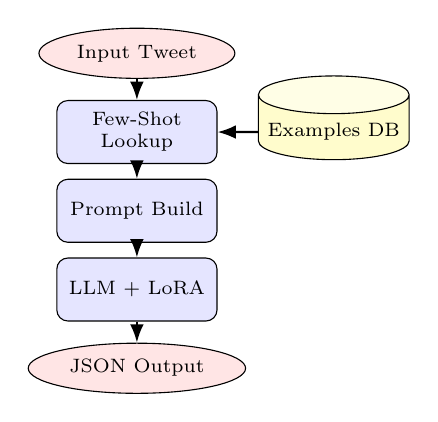
\begin{tikzpicture}[
    node distance=1cm,
    auto,
    block/.style={
        rectangle,
        draw,
        fill=blue!10,
        text width=1.8cm,
        text centered,
        rounded corners,
        minimum height=0.8cm,
        font=\scriptsize
    },
    cloud/.style={
        draw,
        ellipse,
        fill=red!10,
        minimum height=0.6cm,
        font=\scriptsize
    },
    database/.style={
        cylinder,
        cylinder uses custom fill,
        cylinder body fill=yellow!20,
        cylinder end fill=yellow!10,
        shape border rotate=90,
        draw,
        aspect=0.25,
        minimum height=1cm,
        text centered,
        font=\scriptsize
    },
    line/.style={
        draw,
        -Latex,
        thick
    }
]

% Nodes
\node [cloud] (input) {Input Tweet};
\node [block, below of=input] (lookup) {Few-Shot Lookup};
\node [database, right of=lookup, node distance=2.5cm] (db) {Examples DB};
\node [block, below of=lookup] (prompt) {Prompt Build};
\node [block, below of=prompt] (llm) {LLM + LoRA};
\node [cloud, below of=llm] (output) {JSON Output};

% Edges
\path [line] (input) -- (lookup);
\path [line] (db) -- (lookup);
\path [line] (lookup) -- (prompt);
\path [line] (prompt) -- (llm);
\path [line] (llm) -- (output);

\end{tikzpicture}
\captionof{figure}{Stance Detection System Architecture}
\label{fig:architecture}
\end{center}
\vspace{0.5em}

\section{Results}
%This section reports the results of our qualitative and quantitative analysis of influencer discourse. The analysis covers 680,847 tweet-aspect pairs across 38 political aspects, with influencers categorized by political polarizaton into Pro-Ruling (462 influencers) and Pro-Opposition (498 influencers) groups.%% 
{\color{blue} This section reports the results of our qualitative and quantitative analysis of influencer discourse. The original corpus comprised 7.1 million retweets from 960 unique influencers across the 2020--2023 period (Table~\ref{tab:dataset_stats}). After aspect-based filtering---extracting only tweets containing the 35 polar aspects identified in the Methodology---the final dataset comprises 457,509 tweet-aspect pairs (303,233 English and 154,276 Hindi). These pairs correspond to 418,233 unique tweets, as a single tweet may reference multiple aspects. The analysis covers 674 influencers, categorized by political polarization into Pro-Ruling (372 influencers) and Pro-Opposition (302 influencers) groups. Influencers labelled as ``neutral'' were excluded from this analysis, as we focus specifically on the discourse patterns of politically aligned influencers.}
\subsection{Model Performance}
We compare the performance of our Mistral-7B based stance classification approaches against the baseline architectures as described in the Methodology. Figure~\ref{fig:model_comparison} illustrates the comparative results across key metrics. The LoRA-tuned Mistral model consistently outperforms the baseline approaches in all of the metrics (accuracy: 78\%, F1 score (weighted): 77.1\%) for the 264 held out test samples, demonstrating superior capability in capturing the nuances of political stance. The confusion matrix presented in Figure~\ref{fig:confusion_matrix} shows a strong diagonal, indicating high precision in correctly identifying the three stance labels. %Notably, the model effectively minimizes confusion between opposing stances (Favor vs. Against), which is critical for accurate polarization analysis. 
We observe that the instances of misclassification are primarily concentrated around the Neutral category, reflecting the inherent ambiguity often present in less explicit partisan expressions. We present our analysis of these misclassifications in the Discussion section.%, followed by RoBERTa. For the current dataset, we find that PyABSA performs the worst and fails to capture the linguistic nuances of the tweets. 
% In the Appendix, we qualitatively compare the performance of the best and worst performing models, and discuss cases where PyABSA fails to perform for stance classification.
\begin{figure}[H]
  \centering
  \includegraphics[width=0.95\linewidth]{results_eng/model_comparison.png}
  \caption{Performance comparison of the fine-tuned Mistral (LoRA) model against baseline architectures.}
  \label{fig:model_comparison}
\end{figure}
These experiments clearly echo the superior performance of fine-tuned SLMs over the classical transformer based approaches, owing to fine-tuning of the SLM to learn context specific lingusitic attributes. The SLM further outperforms the baseline BERT-based model trained on the same dataset, due to its greater capacity and representational complexity. However, since stance classification is heavily contextual, and the results might vary depending on the data under consideration. We use the best performing LoRA-tuned model for stance classification hereinafter. 
\begin{figure}[H]
  \centering
  \includegraphics[width=0.95\linewidth]{results_eng/mistral_finetuned_confusion_matrix.png}
  \caption{Confusion matrix for the fine-tuned Mistral model on the held-out test set.}
  \label{fig:confusion_matrix}
\end{figure}
%% Detailed Evaluation Results - Moved from Methodology per reviewer comment (Anirban Sen, 6 Jan)
{\color{blue}
% \subsubsection{Detailed Evaluation Metrics}
% Table~\ref{tab:eval_overall_results} presents the detailed metrics for the best performing model (LoRA-adapted Mistral). The model demonstrates competitive performance, effectively balancing precision and recall across classes.

% \vspace{0.5em}
% \begin{center}
% \footnotesize
% \captionof{table}{Stance Classification Evaluation Results (Mistral LoRA)}
% \label{tab:eval_overall_results}
% \begin{tabular}{lr}
% \toprule
% \textbf{Metric} & \textbf{Value} \\
% \midrule
% Total test samples & 264 \\
% Accuracy & 78.0\% \\
% Precision (macro) & 77.6\% \\
% Recall (macro) & 75.3\% \\
% F1-Score (macro) & 76.1\% \\
% F1-Score (weighted) & 77.7\% \\
% \bottomrule
% \end{tabular}
% \end{center}
% \vspace{0.5em}
% Table~\ref{tab:eval_perclass_results} shows per-class performance for the fine-tuned SLM. The model performs strongest on the ``favor'' class (F1=0.82), followed by ``against'' (F1=0.79). The ``neutral'' class shows lower recall (0.60), reflecting the inherent difficulty of distinguishing neutral stances from weakly expressed opinions. We present a detailed analysis of the misclassifications in the Discussion section.
% \begin{center}
% \footnotesize
% \captionof{table}{Per-Class Classification Performance (Mistral LoRA)}
% \label{tab:eval_perclass_results}
% \begin{tabular}{lrrrr}
% \toprule
% \textbf{Class} & \textbf{Precision} & \textbf{Recall} & \textbf{F1} & \textbf{Support} \\
% \midrule
% Against & 0.78 & 0.80 & 0.79 & 95 \\
% Favor & 0.79 & 0.86 & 0.82 & 111 \\
% Neutral & 0.76 & 0.60 & 0.67 & 58 \\
% \bottomrule
% \end{tabular}
% \end{center}
% \vspace{0.5em}
Table~\ref{tab:eval_aspect_results} presents the top 10 per-aspect accuracy for the seed aspects, showing that some yield clearer stance signals than others. aspects like \textit{Modi} (name of the Prime Minister of India) achieve the highest accuracy (94.4\%), followed by \textit{CAA} (89.5\%) and \textit{Congress} (88.9\%) (the largest party in opposition), indicating their usage in tweets with clear stance signatures.

\vspace{0.5em}
\begin{center}
\footnotesize
\captionof{table}{Per-aspect Classification Accuracy (Top 10)}
\label{tab:eval_aspect_results}
\begin{tabular}{lrr}
\toprule
\textbf{aspect} & \textbf{Accuracy} & \textbf{F1 (macro)} \\
\midrule
modi & 94.4\% & 0.91 \\
caa & 89.5\% & 0.90 \\
congress & 88.9\% & 0.84 \\
hindutva & 85.7\% & 0.84 \\
new\_parliament & 85.7\% & 0.82 \\
rahulgandhi & 81.2\% & 0.82 \\
farmers\_protests & 80.0\% & 0.82 \\
muslim & 78.9\% & 0.79 \\
shaheen\_bagh & 78.9\% & 0.71 \\
china & 73.7\% & 0.64 \\
\bottomrule
\end{tabular}
\end{center}
\vspace{0.5em}
}

%% ============================================================
%% SECTION 5.2: MULTILINGUAL STANCE TRENDS
%% ============================================================
{\color{blue}
To evaluate the generalization capability of the fine-tuned model beyond the seed aspects used during training, we conducted a qualitative accuracy check on 20 additional political aspects (out-of-distribution testing) that were not part of the fine-tuning dataset. For each aspect, we randomly sampled 20 tweets and obtained human annotations (by three independent annotators) for stance classification. The model predictions were then compared against these human annotations to assess performance on unseen political topics.

% Across 390 annotated tweet-aspect pairs spanning 20 aspects, the model achieved an overall accuracy of 73.1\%, with a macro F1-score of 65.3\% and weighted F1-score of 70.9\%. Table~\ref{tab:post_analysis_overall} summarizes the overall performance metrics.
% \begin{center}
% \footnotesize
% \captionof{table}{Post-Analysis Accuracy: Overall Metrics}
% \label{tab:post_analysis_overall}
% \begin{tabular}{lr}
% \toprule
% \textbf{Metric} & \textbf{Value} \\
% \midrule
% Total annotated samples & 390 \\
% Accuracy & 73.1\% \\
% Precision (macro) & 68.9\% \\
% Recall (macro) & 66.2\% \\
% F1-Score (macro) & 65.3\% \\
% F1-Score (weighted) & 70.9\% \\
% \bottomrule
% \end{tabular}
% \end{center}
The per-class analysis reveals that the model performs best on the ``against'' stance (F1=0.83), followed by ``favor'' (F1=0.74), while ``neutral'' classification remains challenging (F1=0.40) due to lower recall (29.4\%), suggesting that neutral stance detection remains inherently difficult across both seen and unseen aspects.
% \begin{center}
% \footnotesize
% \captionof{table}{Post-Analysis Accuracy: Per-Class Performance}
% \label{tab:post_analysis_perclass}
% \begin{tabular}{lrrrr}
% \toprule
% \textbf{Class} & \textbf{Precision} & \textbf{Recall} & \textbf{F1} & \textbf{Support} \\
% \midrule
% Favor & 0.67 & 0.82 & 0.74 & 102 \\
% Against & 0.79 & 0.87 & 0.83 & 203 \\
% Neutral & 0.61 & 0.29 & 0.40 & 85 \\
% \bottomrule
% \end{tabular}
% \end{center}
Table~\ref{tab:post_analysis_aspects} presents the per-aspect accuracy for the 20 evaluated aspects. Notable high-accuracy aspects include \textit{Bhakts} (95\%), \textit{Islamists} (95\%), \textit{Democracy} (90\%), \textit{Demonetisation} (90\%), and \textit{Suicides} (90\%). These aspects tend to have clearer partisan framing patterns that the model successfully captures. Conversely, aspects like \textit{MSP} (30\%), \textit{Minorities} (50\%), and \textit{Lynching} (55\%) show lower accuracy, likely due to more nuanced or contested discourse patterns that differ from the training distribution.
\begin{center}
\scriptsize
\captionof{table}{Post-Analysis Accuracy: Per-aspect Performance}
\label{tab:post_analysis_aspects}
\begin{tabular}{lrrr}
\toprule
\textbf{aspect} & \textbf{Samples} & \textbf{Accuracy} & \textbf{F1 (macro)} \\
\midrule
Bhakts & 20 & 95.0\% & 0.65 \\
Islamists & 20 & 95.0\% & 0.33 \\
Democracy & 20 & 90.0\% & 0.61 \\
Demonetisation & 20 & 90.0\% & 0.62 \\
Suicides & 20 & 90.0\% & 0.80 \\
Aatmanirbhar Bharat & 21 & 85.7\% & 0.84 \\
GDP & 20 & 80.0\% & 0.72 \\
Dictatorship & 19 & 78.9\% & 0.43 \\
Inflation & 20 & 75.0\% & 0.66 \\
Ayodhya & 20 & 70.0\% & 0.69 \\
Mahotsav & 20 & 70.0\% & 0.69 \\
Sangh & 20 & 70.0\% & 0.59 \\
Sharia & 20 & 70.0\% & 0.43 \\
Spyware & 20 & 70.0\% & 0.62 \\
Unemployment & 20 & 70.0\% & 0.57 \\
Hathras & 20 & 65.0\% & 0.41 \\
Lynching & 20 & 55.0\% & 0.36 \\
Balochistan & 10 & 50.0\% & 0.24 \\
Minorities & 20 & 50.0\% & 0.46 \\
MSP & 20 & 30.0\% & 0.31 \\
\bottomrule
\end{tabular}
\end{center}
The results demonstrate that while the fine-tuned model generalizes reasonably well to unseen political aspects (73.1\% overall accuracy), performance varies significantly across aspects. Aspects with clearer ideological positioning and less ambiguous framing tend to yield higher accuracy, while aspects involving contested narratives or requiring deeper contextual understanding show reduced performance. This suggests potential avenues for further model improvement through targeted data augmentation.}
\subsection{Partisanship in Influencer Discourse}
Figure~\ref{fig:multilingual_stack} presents stacked stance distribution plots for English and Hindi tweets, for the different aspects considered. We discuss in this section the results for a few example aspects across the polarity spectrum, and present the plots for the rest of the 29 aspects in the appendix.%-- while some of these aspects are highly polar (e.g., Hindutva), some others are relatively less polar (e.g., Democracy), when it comes to influencer discourse as can be seen from table XXX.
The visualization shows three distinct bands/rows of aspects. The top row highlights aspects that the ruling dispensation disproportionately favors in public discourse, while the opposition generally criticizes  (\textit{Hindutva, Modi, etc.}). The middle row represents a "mixed" zone where both the establishment and the opposition show relatively similar stance distributions, indicating areas of shared narrative or lower polarization. The bottom row serves as the counterpart to the first, showcasing aspects that the opposition disproportionately favors and the ruling party generally criticizes (e.g., Rahul Gandhi, Farmer's Protests, etc.). 

A few striking trends emerge. We see that the influencer tweets are significantly partisan and highly correlated to influencer polarity, when it comes to discussion on aspects leaning towards a certain party. As can be seen from the plot, aspects like \textit{Hindutva, Modi,} and \textit{Ram Mandir} are reported with an overwhelmingly positive stance by pro-ruling influencers (and negatively by pro-opposition influencers). Notably, these aspects are also prominently and favorably framed by the ruling establishment across mainstream media and broader public discourse [ref], while being criticized by the opposition.

On the other hand, aspects like \textit{Rahul Gandhi, Muslims, and Farmers' Protests} are reported with a disproportionately negative stance by pro-ruling influencers (and positively by pro-opposition). Once again, the trends closely follow the public discourse around these topics by the political parties the influencers favor [ref].

We assess the statistical significance of the differences between the proportions of tweets expressing favorable and opposing stances for each aspect. An XXX test yields XXX values in the range [XXX–XXX], indicating a high level of statistical significance. The differences between favoring and opposing stances for pro-ruling and pro-opposition groups are also statistically significant, with values in the range [XXX–XXX].


{\color{blue}
\subsubsection{Significance Testing: Binomial GLM Analysis}
To rigorously test whether influencer political alignment significantly predicts the likelihood of expressing a favorable stance toward each aspect, we employ a binomial Generalized Linear Model (GLM) with a logit link function. For each aspect $k$, we model the probability $p_i$ that influencer $i$ tweets favorably as:
\begin{equation}
\text{logit}(p_i) = \beta_0 + \beta_1 \cdot \text{Alignment}_i
\end{equation}
where $\text{Alignment}_i = 0$ for pro-ruling influencers and $\text{Alignment}_i = 1$ for pro-opposition influencers. The response variable is the binomial count $[n_{\text{favor}}, n_{\text{total}} - n_{\text{favor}}]$ per influencer, representing the number of favor tweets out of total tweets for that aspect. A significant $\beta_1$ coefficient ($p < 0.05$) indicates that influencer alignment is a significant predictor of favorable stance expression.

Across 36 aspects tested, 31 (86.1\%) yield statistically significant results ($p < 0.05$), confirming that influencer political alignment is a robust predictor of stance across most political topics. The odds ratios, calculated as $e^{|\beta_1|}$, quantify the magnitude of this effect. Aspects exhibiting the strongest pro-ruling bias include \textit{New Parliament} (OR = 40.76, $p < 10^{-41}$), \textit{Demonetisation} (OR = 34.62, $p < 10^{-36}$), \textit{Aatmanirbhar} (OR = 28.50, $p < 10^{-37}$), and \textit{Ram Mandir} (OR = 25.88, $p < 10^{-84}$). Conversely, aspects with the strongest pro-opposition bias include \textit{Farmers Protests} (OR = 15.78, $p < 10^{-51}$), \textit{Muslim} (OR = 12.07, $p \approx 0$), \textit{Rahul Gandhi} (OR = 10.79, $p \approx 0$), and \textit{Shaheen Bagh} (OR = 10.55, $p < 10^{-70}$). Only five aspects—Suicides, Lynching, Dictatorship, Sharia, and Islamists—show no significant alignment effect, likely due to insufficient sample sizes or low variation in stance across political groups.

Figure~\ref{fig:forest_plot} presents a forest plot visualization of these results. The x-axis displays odds ratios on a logarithmic scale, with the vertical line at OR = 1 representing no effect. Points to the left indicate aspects where pro-ruling influencers are more likely to favor (red), while points to the right indicate pro-opposition favor (blue). Horizontal lines represent 95\% confidence intervals. The plot reveals a clear bimodal distribution: aspects cluster either strongly to the left (pro-ruling favor) or strongly to the right (pro-opposition favor), with very few aspects near the center. This visual pattern reinforces the quantitative finding that Indian political influencer discourse is deeply polarized, with stance expression on most political topics being predictable from influencer alignment alone.
\begin{figure}[H]
  \centering
  \includegraphics[width=0.95\linewidth]{results_eng/1_forest_plot_odds_ratio.png}
  \caption{Forest plot showing odds ratios with 95\% confidence intervals for the effect of influencer alignment on favorable stance expression. Red points indicate aspects where pro-ruling influencers are significantly more likely to favor; blue points indicate pro-opposition favor; gray points are non-significant.}
  \label{fig:forest_plot}
\end{figure}
}

Additionally, the stance distribution patterns are remarkably similar across both languages as can be seen from the plot. A statistical significance test yields values in the range [XXX–XXX] for the differences in tweet proportions between English and Hindi across each stance category.This observation suggests that the polarization dynamics and narrative structures deployed by political influencers are consistent, irrespective of the linguistic medium. We further corroborate this finding by cross-referencing it with a negativity scatter analysis (Figure~\ref{fig:negativity_scatter}).%, which similarly indicated high congruence in the sentiment and negativity levels associated with specific aspects across both languages.
\begin{figure}[H]
  \centering
  \includegraphics[width=0.95\linewidth]{results_eng/combined_hindi_english_stance_stacked.png}
  \caption{Stacked stance distribution comparison between English and Hindi tweets.}
  \label{fig:multilingual_stack}
\end{figure}

%Given this high degree of congruence between English and Hindi discourse, we appended the two datasets for the remainder of our analysis to provide a more comprehensive view of the political landscape.
\begin{figure}[H]
  \centering
  \includegraphics[width=0.95\linewidth]{results_eng/6_negativity_scatter.png}
  \caption{Comparison of negativity scores for aspects in English vs. Hindi tweets.}
  \label{fig:negativity_scatter}
\end{figure}
The scatter plot in Figure~\ref{fig:negativity_scatter} plots the average percentage of \textit{against} stance (termed as the \textit{negativity score}) for each aspect in English (X-axis) against its score in Hindi (Y-axis). We observe a strong positive correlation, with most aspects clustering along the diagonal ($y=x$ line). To understand the significance of these results, we calculate the Root Mean Squared Error (RMSE) and Mean Absolute Error (MAE). For Pro-Ruling aspects ($n=32$ aspects), we obtain: RMSE = 5.11, and MAE = 3.76 percentage points are obtained. For Pro-Opposition aspects ($n=33$ aspects): RMSE = 7.37, and MAE = 4.89 percentage points are obtained. These significantly low error values confirm that the cross-lingual negativity patterns are highly consistent, further supporting the aggregation of English and Hindi datasets for subsequent analysis.

% {\color{blue}
% To quantify the cross-lingual consistency, we measure the perpendicular distance of each data point from the diagonal ($y=x$) line. For a point $(x_i, y_i)$ representing the negativity scores in English and Hindi respectively, the perpendicular distance to the diagonal is given by:
% \[
% d_i = \frac{y_i - x_i}{\sqrt{2}}
% \]
% We then compute the following metrics over all $n$ aspects: (1) \textbf{Root Mean Squared Error (RMSE)}: $\text{RMSE} = \sqrt{\frac{1}{n}\sum_{i=1}^{n}d_i^2}$, which captures the average magnitude of deviation, penalizing larger deviations more heavily; (2) \textbf{Mean Absolute Error (MAE)}: $\text{MAE} = \frac{1}{n}\sum_{i=1}^{n}|d_i|$, which provides the average absolute deviation from the diagonal; (3) \textbf{Median Absolute Distance}: the median of $|d_i|$, a robust measure less sensitive to outliers; and (4) \textbf{Mean Signed Distance}: $\frac{1}{n}\sum_{i=1}^{n}d_i$, which indicates systematic bias (positive values suggest higher negativity in Hindi, negative values suggest higher negativity in English).

% For Pro-Ruling aspects ($n=32$ aspects), we obtain: RMSE = 5.11 percentage points, MAE = 3.76 pp, Median Absolute Distance = 2.39 pp, and Mean Signed Distance = +1.01 pp (slight Hindi bias). For Pro-Opposition aspects ($n=33$ aspects): RMSE = 7.37 pp, MAE = 4.89 pp, Median Absolute Distance = 2.74 pp, and Mean Signed Distance = $-$1.75 pp (slight English bias). These low error values -- with median deviations under 3 percentage points in both camps -- confirm that the cross-lingual negativity patterns are highly consistent, further supporting the aggregation of English and Hindi datasets for subsequent analysis.
% }

The findings indicate that topics evoking negative sentiment in English discourse tend to trigger similar levels of negativity in Hindi, reinforcing the hypothesis of a unified partisan narrative that transcends language barriers. 
{\color{blue}Similar cross-lingual consistency is observed for favorable (RMSE: 5.68–6.09 pp) and neutral (RMSE: 4.33–5.90 pp) stances, confirming that stance distribution patterns are robust across both languages for all stance categories}
The visual evidence suggests that the emotional valence of political topics is consistent across linguistic communities, further justifying the aggregation of datasets for subsequent analysis.

% Using the combined English and Hindi dataset, we next re-examine the percentages of \textit{favor} stance (normalized favor rates) for each of the 38 aspects. Figure~\ref{fig:butterfly_favor} displays these percentages, with Pro-Ruling favor percentages on the right and Pro-Opposition favor percentages on the left.

% \begin{figure}[H]
%   \centering
%   \includegraphics[width=0.95\linewidth]{results_eng/2_butterfly_favor_normalized.png}
%   \caption{Butterfly chart showing normalized favor rates by aspect (combined English \& Hindi data).}
%   \label{fig:butterfly_favor}
% \end{figure}

% The combined analysis reinforces the bimodal nature of the discourse. We observe a set of aspects where the Pro-Ruling side exhibits near-complete dominance in favorable expression, contrasting sharply with aspects where the Pro-Opposition side dominates. Topics located near the center of the chart continue to exhibit more balanced favor distributions, but the overall trend confirms that most political topics in the Indian context are heavily skewed toward one side's narrative. This polarization is even more pronounced when leveraging the larger, combined dataset, validating the robustness of our initial findings.
\subsection{Aspect-Level Polarization}
Figure~\ref{fig:divergence_scatter} presents the aspect level stance divergence for the combined corpus, for all aspects. This scatter plot maps each aspect based on the difference between percentage of favor tweets (x-axis) and against tweets (y-axis). The size of each bubble represents the number of tweets for a certain aspect. The color gradient represents the ``favor divergence score" -- the difference between percentages of favor and against tweets (green representing high \textit{favor} percentage, and red representing high \textit{against} percentage).
\begin{figure}[H]
  \centering
\includegraphics[width=0.95\linewidth]{results_eng/divergence_scatter_english_hindi_combined.png}
  \caption{aspect-level stance divergence scatter plot for the combined English and Hindi dataset.}
  \label{fig:divergence_scatter}
\end{figure}
The plot clearly highlights the two distinct poles occupied by the different aspects. We find two clusters of highly polar aspects in the first and third quadrants of the plot. These are aspects where one side of influencers (pro-ruling/pro-opposition) is disproportionately in favor. %Outliers in this plot represent topics that generate unique polarization patterns -- for instance, topics where one side is highly favorable while the other is not necessarily hostile but silent, or where both are hostile (bottom-left). 
We also see relatively \textit{neutral} (yellow) aspects in the middle. However, the bubble sizes for these neutral aspects are significantly smaller, indicating their scarcity in influencer discourse. Thus, we see a highly polar aspect level discourse -- specific high-volume topics drive the bulk of the polarization and are discussed in a highly partisan manner, while a "long tail" of insignificantly discussed issues remain relatively contested or neutral. %\footnote{We also present a plot of the variation in favor divergence with aspect size (number of tweets) in the Appendix, which exhibits a similar finding where neutral aspects are seen to clutter near the origin, indicative of their relative insignificance in the influencer discourse.}

%% ============================================================
%% SECTION 5.5: COMPLETE STANCE DISTRIBUTION
%% ============================================================
% \subsection{Complete Stance Distribution by aspect}
% Figure~\ref{fig:stance_by_aspect} presents the full stance distribution for each aspect, disaggregated by political affiliation. Each aspect displays proportions of favor, neutral, and against stances for both Pro-Ruling and Pro-Opposition influencers.

% \begin{figure}[H]
%   \centering
%   \includegraphics[width=0.95\linewidth]{results_eng/4_stance_distribution_by_aspect.png}
%   \caption{Stance distribution by aspect and political affiliation, showing proportions of favor, neutral, and against stances.}
%   \label{fig:stance_by_aspect}
% \end{figure}
% To organize aspects into meaningful thematic categories, we employed Google's Gemini model. The model was provided only with the list of 38 aspects and prompted to create thematic buckets based on its knowledge of Indian political discourse. Table~\ref{tab:stance_composition} presents the resulting aspect categories.
% \begin{center}
% \footnotesize
% \captionof{table}{aspects Grouped by Thematic Category (Generated using Gemini)}
% \label{tab:stance_composition}
% \begin{tabular}{p{2.4cm}p{4.1cm}}
% \toprule
% \textbf{Category} & \textbf{aspects} \\
% \midrule
% Favor-dominant (both) & ayodhya, mahotsav, ucc \\
% Against-dominant (both) & inflation, unemployment, suicides \\
% Split (PR favor, PO against) & modi, ram\_mandir, aatmanirbhar, hindutva, farm\_laws, caa \\
% Split (PO favor, PR against) & rahulgandhi, congress, farmers\_protests, shaheen\_bagh, muslim \\
% Mixed neutral ($>$20\%) & china, gdp, democracy, minorities \\
% \bottomrule
% \end{tabular}
% \end{center}
% {\footnotesize \textit{Note: PR = Pro-Ruling, PO = Pro-Opposition}}
{\color{blue}
\subsubsection{Thematic Stance Analysis}
To perform a thematic analysis of stance, we employed ChatGPT (GPT-4.5\footnote{We also tried Gemini for this exercise, but a manual analysis revealed a slightly better performance of GPT, with clearer aspect definitions.}) with a detailed prompt (appendix) through few-shot learning -- the model was provided with the list of aspects and a sample of tweets for each aspect, and instructed to: (A) read all tweets to understand framing patterns, tone, and narrative structures; (B) create high-level thematic buckets that capture major stance/framing themes relevant to pro-ruling vs. pro-opposition influencer discourse; (C) assign each aspect to one primary bucket with reasoning grounded in observed tweet patterns.

This process yielded nine thematic buckets: (1) \textit{Leader \& Party Contestation} (modi, rahulgandhi, congress); (2) \textit{Institutions, Democracy \& State Accountability} (democracy, dictatorship, spyware, new parliament); (3) \textit{Economy, Development \& Macro-Stewardship} (aatmanirbhar, demonetisation, gdp, inflation, unemployment, suicides); (4) \textit{Agrarian Reform \& Farmer Movement} (farm laws, farmers protests, msp); (5) \textit{Citizenship, Belonging \& Mass Protest Politics} (caa, shaheen bagh); (6) \textit{Majoritarian Ideology \& Hindu Nationalist Mobilization} (hindutva, sangh, bhakts, hindu); (7) \textit{Communal Relations, Minority Rights \& Collective Violence} (minorities, muslim, lynching, sharia, islamists, hathras); (8) \textit{Symbolic Nationhood \& Cultural-Religious Projects} (ayodhya, ram mandir, mahotsav); and (9) \textit{Security, Territory \& Geopolitics} (china, kashmir, balochistan, kashmiri pandits).

Figure~\ref{fig:party_focus_stance} presents the stance analysis for each thematic bucket, for pro-ruling and pro-opposition influencers. Each horizontal bar represents the percentage of a side's total tweets devoted to a given bucket.
\begin{figure}[H]
  \centering
  \includegraphics[width=0.95\linewidth]{results_eng/party_focus_stance_breakdown.png}
  \caption{Thematic stance analysis: Bar length indicates percentage of total tweets}
  \label{fig:party_focus_stance}
\end{figure}
Several differences emerge between the two camps, in terms of the partisanship exhibited at a theme level. \textit{Leader \& Party Contestation} dominates both groups' discourse, but occupies a larger share for Pro-Opposition (59.3\%) than Pro-Ruling (49.7\%). Pro-Ruling influencers allocate a higher proportion to \textit{Majoritarian Ideology \& Hindu Nationalist Mobilization} (16.8\%) compared to Pro-Opposition (9.3\%). \textit{Symbolic Nationhood \& Cultural-Religious Projects} accounts for 4.5\% of Pro-Ruling discourse but only 0.8\% of Pro-Opposition discourse. Conversely, \textit{Institutions, Democracy \& State Accountability} receives greater attention from Pro-Opposition (4.1\%) than Pro-Ruling (1.9\%). The stance composition within buckets also differs: Pro-Ruling tweets in the \textit{Majoritarian Ideology} and \textit{Leader and Party Contestation} buckets are predominantly favorable (green), while Pro-Opposition tweets in the same buckets are predominantly against (red). A detailed table showing individual thematic bucket definitions, aspect contributions to each bucket, with stance breakdowns and tweet counts, is provided in the Appendix.}
{\color{blue}
\subsection{Misclassification}
We discuss the common sources of misclassification for our best performing model in this section. We found that a common source of error involves implicit evaluation, especially in tweets discussing economic indicators such as GDP, exports, or inflation. Although these tweets appear factual, human annotators interpreted them as favourable because such statistics are commonly used to signal government performance or national strength. The model, however, often treats numeric information as neutral and fails to recognise the intent behind these references. Another frequent issue relates to sarcasm and mockery, especially when expressed through quotation marks, rhetorical framing, or code-mixed language. Tweets invoking ironic references to ``democratic'' governance, written with a mix of Hindi and English or employing historical analogy are frequently misclassified. In these cases, surface-level language appeared neutral or even positive, while the intended stance was oppositional. This highlights the difficulty of capturing pragmatic cues that rely on shared political and cultural context. Misclassification also occurs due to unclear targets of critique. Some tweets mention politically charged events but direct criticism toward secondary actors such as opposition leaders, institutions, or public figures. The model tends to rely on aspect associations and struggles to distinguish between references to an issue and evaluation of a specific actor. Finally, some errors involve descriptive statements with implicit moral judgement, particularly in tweets reporting violence or governance failures. While the language used is factual, human readers interpret these descriptions as critical. The model, by contrast, often classifies them as neutral due to the absence of explicit sentiment markers.
\begin{center}
\tiny
\captionof{table}{Representative Examples of Model Misclassification}
\label{tab:misclassification_examples}
\begin{tabular}{p{5.5cm}p{1.3cm}ccp{3.5cm}}
\toprule
\textbf{Tweet} & \textbf{Aspect} & \textbf{Model} & \textbf{Human} & \textbf{Reasoning} \\
\midrule
India Exports to Bahrain \$450M... Total exports just 1.5B, India GDP \$2.7T, so not even 0.1\%... The more they overdo the bigger the hit back on local converts. & GDP & Neutral & Favor & Model treats comparative economic statistics as descriptive data, missing implied national strength endorsement. \\
\midrule
6th March is a Sunday please fill your vehicles full tank wait to see the fuel price on the 8th of March \& thank Modiji to have made you aatmanirbhar & aatmanirbhar & Favor & Against & Sarcasm framed as informational statement. \\
\midrule
Vultures of Congress crossing all limit. Now CM @VNarayanasami is giving tribute to Hathras victim using picture of a girl who died 2 years back. & hathras & Against & Neutral & Model anchors on ``Hathras'' aspect even though the stance is on Congress. \\
\midrule
Both police \& relatives of Israr killed by brutal beating by a crowd are avoiding to call it `mob lynching' for reasons best known to them... & lynching & Neutral & Against & Model treats descriptive crime reporting as neutral and misses implicit condemnation. \\
\bottomrule
\end{tabular}
\end{center}
}

\section{Discussion}
We study political discourse of Indian influencers in this paper to understand if they exhibit polarization with respect to various social and political issues. In this direction, we first develop a proxy for their political leaning using the number of political retweets they receive around their tweets. Next, we analyze the stance of their tweets around different aspects, using an SLM fine-tuned on their tweets. Our findings conclusively prove that most Indian influencers are significantly partisan when it comes to their tweets on various aspects. The aggregate partisanism also is dichotomous in nature, wherein there exists two distinct communities of influencers, one in favor of the ruling dispensation and the other against it.

There are several nationally and regionally prominent political parties functioning in India. However, the dichotomy that we observe in the influencer discourse provides concrete indication of the highly bipolar nature of the Indian polity. We see that influencers with a significant political leaning towards the ruling dispensation disproportionately favor issues like \textit{Hindutva, Hinduism, Kashmiri Pandits} and write against \textit{farmer's protests, muslims, bharatjodoyatra}. On the other hand, the pro-opposition influencers follow the exact opposite trend around the same issues. We thus see a clear trend of influencers kotowing their favorite party lines. With the recent trend of increasing religious and political polarization in India [ref], this especially does not augur well. Influencers are highly popular figures, many of whom are revered and closely followed on social media by numerous users. A bipolar nature of the influencer discourse thus amplifies the extant biases in the society, thereby leading to a fragmented democracy. 

We also see that these trends are uniformly observed for both English and Hindi tweets, indicative of the fact that the observed polarization holds across languages. In a country where a significant fraction of the social media population consumes tweets in Hindi [ref], this is a sign of a polarized political discourse cutting across linguistic borders.

The topical analysis of tweets reveals ...

This work comes as a timely intervention around influencer polarization in India, provided that several recent studies have targeted similar research questions. Our work acts as a formative step towards large-scale analysis of influencer discourse on social media (from 2020-2023). A major contribution of this study is the development of a generalizable research framework to study aspect based stance on social media. While we study influencer discourse in India corresponding to two languages, the framework is applicable to any geography and can be extended to work on other languages as well. The use of an SLM to perform stance analysis also highlights the need to incorporate low-infrastructure methods to perform large-scale data analysis.

As part of future work, we intend to extend the study to other regional languages in India, to see if similar trends are observed. Furthermore, while the current work focuses on an overall analysis of influencer discourse, a temporal study capturing the evolution of influencer leaning and discourse partisanism can be undertaken. The current study only considers influencer tweets that have received at least one political retweet (retweet by a politician). However, it would be interesting to include other tweets on similar aspects, followed by a stance analysis. A comparative analysis of the trends can then provide us with stronger empirical evidence of partisanism in tweets, irrespective of the political endorsements received by them.

\section{Conclusion}
In this paper, we examined the political discourse of Indian influencers to assess the extent and nature of polarization across a range of social and political issues. To this end, we first proposed a proxy to infer influencers’ political leanings based on the political retweets received in response to their content. We then analyzed the stances expressed in their tweets with respect to different issue-specific aspects, leveraging a small language model fine-tuned on influencer-generated data. Our analysis provides strong empirical evidence that a majority of Indian influencers exhibit pronounced partisanship in their engagement with these issues. Furthermore, polarization at the aggregate level is distinctly dichotomous, revealing the presence of two well-defined communities of influencers—one broadly aligned with the ruling dispensation and the other positioned in opposition. These findings highlight the influential role of content creators in shaping and reinforcing polarized political discourse on social media platforms.


% TODO: Add discussion content

\section{Conclusion}

% TODO: Add conclusion content

\section*{Acknowledgment}

We thank Professor Joyojeet Pal for providing the tweet dataset used in this research, and Ashoka University for supporting this work.


\end{multicols}
\bibliographystyle{plainnat}
\bibliography{bibliography}
\end{document}
